% Provenance (never printed): enseignement scientifique premiere (2019),
% theme "La Terre, un astre singulier: la forme de la Terre" (Eratosthenes,
% meridian measurement by triangulation, the metre); see
% sources/book2/PROVENANCE.md. Every length on the ellipsoid is computed in
% figdata/grade-10/meridian_degree.py (WGS 84, ledger wgs84:ellipsoid).
\chapter{测量地球}\label{ch:g10:measuring-the-earth}

在海滩上站立，看着一艘船驶向远方的大海。它并不是简单地缩小到看不见为止：
先是船身消失，仿佛沉入水中，接着是上层建筑的下部，
最后才是桅杆的顶端。
你与船之间的海面并不平坦，而是向外隆起。
两千二百多年前，亚历山大城的一位学者
把类似的观察——正午影子的长度——变成了对整个星球大小的测量。
本章讲述这一测量及其后的各次测量：
测量员在各国之间铺设的\omterm{def:g10:measuring-the-earth:triangulation}{三角测量}网，
为查明地球是否扁平而派往北极和赤道的考察，
米的诞生，
以及今天借以测量地球的卫星。

\begin{omfigure}
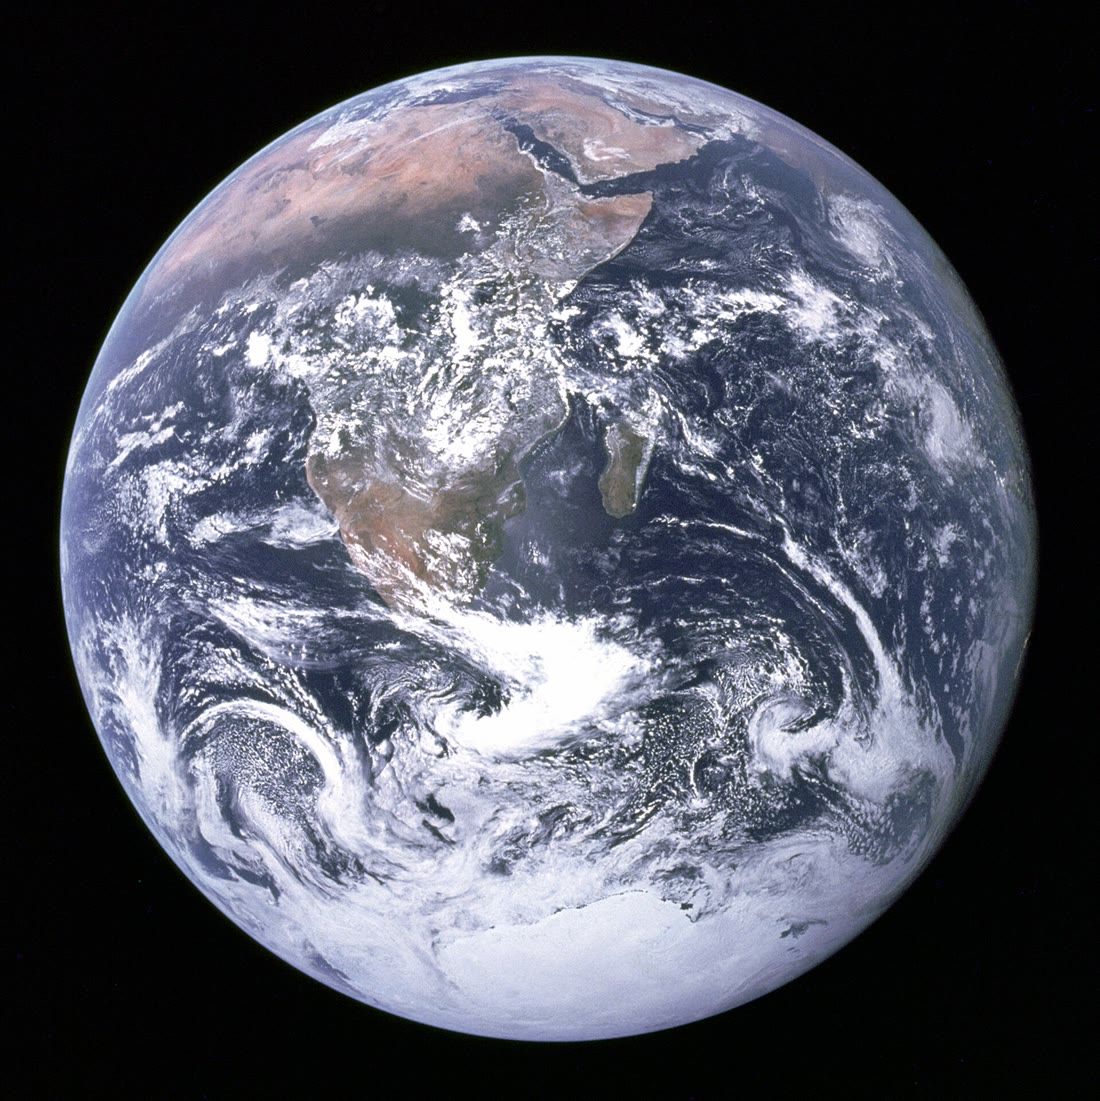
\includegraphics[width=0.5\linewidth]{images/book2/g10-nasa-apollo17-earth.jpg}

{\small 阿波罗~17 号飞船机组在前往月球途中拍摄的地球，
时间为 1972 年 12 月。画面中有非洲、阿拉伯半岛和南极洲的冰原。照片：
NASA（公有领域）。}
\end{omfigure}

\begin{recall}
地球上某地的位置由纬度和经度确定。纬度是该地位于赤道以北或以南的角度，
经度是该地位于参考经线以东或以西的角度；
经线连接两极，纬线与赤道平行，绕地球一周（见第 1 册）。
在均匀介质中，光沿直线传播，
而来自遥远太阳的光线彼此平行（见物理各册）。
在直角三角形中，锐角的正弦是对边与斜边之比，
余弦是邻边与斜边之比，
正切是对边与
邻边之比（见数学教材）。
\end{recall}

\section{圆形的地球}

早在人们能从太空观察地球之前，
就已有若干观察表明地球是圆的。
\begin{itemize}
  \item \textbf{越过地平线的船。}远去的船总是从下往上消失，
        不论朝哪个方向、在哪片海上：海面
        处处是弯曲的。
  \item \textbf{月球上的影子。}月食期间，地球的影子投在月球上。
        影子的边缘总是一段圆弧，
        无论夜间何时都是如此；只有球体
        才会在各个方向投下圆形的影子。
  \item \textbf{星空随纬度变化。}向北行进的旅行者看到北极星越升越高，
        南天的星星沉入地平线之下：旅行者的
        地平线会随之倾斜——
        他正行走在弯曲的表面上。
  \item \textbf{环球航行与太空视角。}船只，继而是飞机，已朝各方向环绕世界航行；
        1960 年代起，
        整个圆球形的地球已被拍摄下来。
\end{itemize}

\begin{omfigure}
\begin{tikzpicture}[font=\small, >={Stealth[length=2.2mm]}]
  % sea surface: arc of a circle of radius 8 centred at (0,-8) (curvature exaggerated)
  \fill[omDef!10] plot[domain=-4.6:4.6, samples=60] (\x,{sqrt(64-\x*\x)-8}) -- (4.6,-2.2) -- (-4.6,-2.2) -- cycle;
  \draw[omDef!70!black, thick] plot[domain=-4.6:4.6, samples=60] (\x,{sqrt(64-\x*\x)-8});
  % observer on a small tower at x=-4 (surface y=-1.072), eye at y=-0.235
  \draw[black!70, line width=1pt] (-4,-1.072) -- (-4,-0.235);
  \fill (-4,-0.235) circle (2pt);
  \node[anchor=east, align=right] at (-4.1,-0.2) {观察者的 \\眼睛};
  % line of sight tangent at x=-0.5 (y=-0.0156, slope 0.0626)
  \draw[omThm!80!black, thick] (-4,-0.235) -- (4.4,0.290);
  \node[omThm!80!black, anchor=south, rotate=3.6] at (1.3,0.1) {视线};
  \fill[omThm!80!black] (-0.5,-0.0156) circle (1.4pt);
  % ship at x=3 (surface y=-0.584), tilted 22 degrees with the local vertical
  \begin{scope}[shift={(3,-0.584)}, rotate=-22]
    \fill[black!12] (-0.6,0) -- (0.6,0) -- (0.75,0.32) -- (-0.75,0.32) -- cycle;
    \draw[black!45, densely dashed] (-0.6,0) -- (0.6,0) -- (0.75,0.32) -- (-0.75,0.32) -- cycle;
    \draw[black!45, densely dashed] (0,0.32) -- (0,0.95);
    \draw[black!80, line width=1pt] (0,0.95) -- (0,1.55);
    \fill[black!80] (0,1.55) -- (0.32,1.25) -- (0,1.25) -- cycle;
  \end{scope}
  \node[anchor=north, align=center, font=\footnotesize] at (2.9,-1.25) {船身与下部桅杆 \\被隆起的海面遮住};
  \node[anchor=north, font=\footnotesize] at (-0.5,-0.1) {地平线};
\end{tikzpicture}

{\small 船为何从下往上消失：观察者只能看到
位于掠过地平线处海面的视线上方的部分。
图中的弯曲程度被大大夸大。}
\end{omfigure}

\section{埃拉托斯特尼测量地球}

昔兰尼的埃拉托斯特尼（前 276--194 年）是亚历山大城的图书馆馆长。他曾听说，
在远离亚历山大城、位于尼罗河上游的塞伊尼（今阿斯旺），
夏至那天正午，太阳把一口水井的整个井底都照亮了：此时
太阳恰好在头顶正上方。同一时刻，亚历山大城一根竖直的木棍
投下一段很短的影子：太阳光线与竖直方向的夹角约为
\qty{7.2}{\degree}，即整个圆周的五十分之一。
% ledger: erat:method, erat:stadion

\begin{omfigure}
\begin{tikzpicture}[font=\small, >={Stealth[length=2.2mm]}]
  \def\R{2.4}
  \fill[omDef!8] (0,0) circle (\R);
  \draw[omDef!70!black, thick] (0,0) circle (\R);
  \coordinate (O) at (0,0);
  \coordinate (S) at (\R,0);
  \coordinate (A) at ({\R*cos(25)},{\R*sin(25)});
  \coordinate (T) at ({(\R+0.75)*cos(25)},{(\R+0.75)*sin(25)});
  \coordinate (T2) at ({(\R+1.75)*cos(25)},{(\R+1.75)*sin(25)});
  % radii
  \draw[black!70] (O) -- (S);
  \draw[black!70] (O) -- (A);
  \draw[black!40, densely dashed] (A) -- (T2);
  \fill (O) circle (1.5pt) node[below left] {圆心};
  % stick at Alexandria, along the radius
  \draw[line width=1.6pt, black!85] (A) -- ($(A)!0.6!(T)$);
  % well at Syene
  \draw[black!80, thick] ({\R-0.38},-0.12) -- (\R,-0.12) ($(S)+(0,0.12)$) -- ({\R-0.38},0.12);
  % parallel sun rays coming from the right
  \foreach \y in {-1.6,-0.8,0.8,1.6} \draw[->, omThm!70, thick] (6.6,\y) -- (4.4,\y);
  \draw[->, omThm!85!black, thick] (6.6,0) -- (\R+0.05,0);
  \draw[->, omThm!85!black, thick] (6.6,{(\R+0.45)*sin(25)}) -- ({(\R+0.45)*cos(25)+0.03},{(\R+0.45)*sin(25)});
  \node[omThm!85!black, align=center, anchor=west] at (4.6,2.35) {阳光：\\平行光线};
  % angles
  \draw[omExo!80!black, thick] (0.75,0) arc (0:25:0.75);
  \node[omExo!80!black] at (1.05,0.22) {$\alpha$};
  \coordinate (Q) at ($(A)!0.6!(T)$);
  \draw[omExo!80!black, thick] ($(Q)+(0.8,0)$) arc (0:25:0.8);
  \node[omExo!80!black] at ($(Q)+({1.08*cos(12.5)},{1.08*sin(12.5)})$) {$\alpha$};
  \node[anchor=east] at ($(A)+(-0.12,0.18)$) {亚历山大城};
  \node[anchor=north west] at ($(S)+(0.3,-0.12)$) {塞伊尼};
  \node[font=\footnotesize, anchor=north] at ($(O)!0.5!(S)+(0.2,-0.05)$) {};
  \draw[<->, black!60] ({(\R-0.3)*cos(3)},{(\R-0.3)*sin(3)}) arc (3:22:{\R-0.3});
  \node[anchor=east, font=\footnotesize] at ({(\R-0.35)*cos(13)},{(\R-0.35)*sin(13)}) {$d$};
\end{tikzpicture}

{\small 埃拉托色尼的推理。在塞伊尼，太阳直射，其光线指向
地心。在亚历山大城，一根竖直的杆子同样指向
地心，它与光线成夹角 $\alpha$。两地之间地心处的角
同为 $\alpha$。图中此角画得夸大了，它实际上
只有 \qty{7.2}{\degree}。}
\end{omfigure}

\begin{proposition}[埃拉托色尼关系]\label{prop:g10:measuring-the-earth:eratosthenes}
若两地位于同一条经线上，相距 $d$，且太阳光线在正午
与竖直方向所成的角相差 $\alpha$（以
度为单位），则地球的周长为
\[
  C = \frac{\qty{360}{\degree}}{\alpha}\, d .
\]
\end{proposition}

\begin{proof}
太阳距离很远，射到两地的光线近似平行。
在每一地点，竖直方向都指向地心。在
图中，射到杆子上的光线与过塞伊尼的半径
是两条平行线，过亚历山大城的半径与二者相交：
杆子与光线之间的角 $\alpha$，与两半径在地心处的夹角，
是一对内错角，因此相等。弧 $d$ 所占
整个圆周的比例，与角 $\alpha$ 占周角的比例相同，
即 $d/C = \alpha/\qty{360}{\degree}$。
\end{proof}

\begin{method}[由两个影子测量周长]\label{met:g10:measuring-the-earth:shadows}
\begin{enumerate}
  \item 在（近似）同一条经线上选取两地，测量两地间的
        南北距离 $d$。
  \item 在同一天当地正午，在每一地点测量竖直杆与
        太阳光线所成的角：$\tan \theta = s/h$，
        其中 $h$ 为杆高，$s$ 为
        影长。切勿直视太阳本身，角度只需由
        影子读出。
  \item 取两个角之差 $\alpha$，并应用
        $C = (360/\alpha)\,d$.
\end{enumerate}
\end{method}

\begin{example}[埃拉托色尼的数值]\label{ex:g10:measuring-the-earth:numbers}
% ledger: erat:method, erat:stadion
埃拉托色尼取亚历山大城到塞伊尼的距离为 5000
\emph{斯塔迪亚}，古希腊的长度单位。取 $\alpha = 1/50$ 个圆周，
\[
  C = 50 \times 5000 = 250\,000 \text{ 斯塔迪亚}.
\]
斯塔迪亚有多长？史学家至今仍有争论。若取
\qty{157.2}{m}，则 $C \approx \qty{39300}{km}$；取 \qty{166.7}{m}，
则 $C \approx \qty{41700}{km}$。经线的真实圆周长为
\qty{40008}{km}：两种取值下，埃拉托色尼的误差都在百分之几之内。
\end{example}

\begin{remark}[所作假设]\label{rem:g10:measuring-the-earth:assumptions}
埃拉托色尼假设地球为球体，太阳距离足够远，使其光线
近似平行；塞伊尼恰好位于回归线上（此处太阳可位于头顶正上方），并且
塞伊尼正位于亚历山大城的正南方。这些假设都只是近似成立：阿斯旺
位于亚历山大城以东约 \qty{3}{\degree} 经度处。关键在于
两地距离中的南北分量，即沿经线方向的那一部分。
% ledger: geonames:aswan, geonames:alexandria
\end{remark}

\section{三角测量}

用测链或测杆在地面上测量长距离既费时，
跨越河流、森林和山地时则根本无法进行。角度则不同，
可用装在刻度圆上的望远镜非常精确地测量，
依次对准两个远处的信号。自十八世纪起，
测量员便用此法测量整个国家。

\begin{definition}[大地测量学]\label{def:g10:measuring-the-earth:geodesy}
\emph{大地测量学}\index{大地测量学}是测量地球的形状和
大小以及地表点位置的科学，并
研究它们随时间的变化。
\end{definition}

\begin{definition}[三角测量]\label{def:g10:measuring-the-earth:triangulation}
\emph{三角测量}\index{三角测量}借助一串
三角形确定远处各点的位置：一条边即\emph{基线}，须在地面上非常仔细地测量；
三角形的所有角均在其顶点处测得，
其余各边随后可由计算求得。
\end{definition}

计算依据的是任意三角形中边与角之间的
一个关系。设三角形 $ABC$，记 $a$、$b$、$c$ 为
与顶点 $A$、$B$、$C$ 相对的边，
并以 $A$、$B$、$C$ 同时表示这些顶点处的角。

\begin{proposition}[正弦定理]\label{prop:g10:measuring-the-earth:sine-rule}
在任意三角形 $ABC$ 中，
\[
  \frac{a}{\sin A} = \frac{b}{\sin B} = \frac{c}{\sin C}.
\]
\end{proposition}

\begin{proof}
过 $C$ 作高，与直线 $AB$ 相交于 $H$（见下图
第二幅小图）；记 $h = CH$。在直角三角形 $AHC$ 中，$\sin A = h/b$，
故 $h = b \sin A$。在直角三角形 $BHC$ 中，$\sin B = h/a$，
故 $h = a \sin B$。由此得 $b \sin A = a \sin B$，即 $a/\sin A = b/\sin B$。
（若角 $B$ 为钝角，则点 $H$ 落在 $B$ 之外，此时直角三角形
在 $B$ 处的角为 $\qty{180}{\degree} - B$，其正弦值相同。）
对过 $A$ 的高作同样的论证，即得 $b/\sin B = c/\sin C$。
\end{proof}

\begin{omfigure}
\begin{tikzpicture}[font=\small, >={Stealth[length=2mm]}]
  \begin{scope}
    \coordinate (A) at (0,0); \coordinate (B) at (2.0,0.25);
    \coordinate (C) at (0.9,1.9); \coordinate (D) at (3.0,2.1);
    \coordinate (E) at (1.9,3.8); \coordinate (F) at (3.9,4.1);
    \coordinate (G) at (2.7,5.6);
    \draw[black!60] (A) -- (C) -- (B) (C) -- (D) -- (B) (C) -- (E) -- (D) -- (F) -- (E) -- (G) -- (F);
    \draw[omThm!85!black, line width=2pt] (A) -- (B);
    \foreach \p in {A,B,C,D,E,F,G} \fill (\p) circle (1.6pt);
    \node[below left] at (A) {$A$}; \node[below right] at (B) {$B$};
    \node[left] at (C) {$C$}; \node[right] at (D) {$D$};
    \node[left] at (E) {$E$}; \node[right] at (F) {$F$}; \node[above] at (G) {$G$};
    \node[omThm!85!black, anchor=north, font=\footnotesize] at (1.25,-0.3) {实测基线};
    \draw[omExo!80!black] ($(A)!0.28!(B)$) arc[start angle=7, end angle=64.6, radius=0.56];
    \draw[omExo!80!black] ($(B)!0.3!(A)$) arc[start angle=187, end angle=123, radius=0.6];
    \draw[black!50, densely dashed] (-0.5,0) -- (-0.5,5.6);
    \draw[->, black!70] (-0.5,5.0) -- (-0.5,5.8) node[above] {北};
    \node[rotate=90, font=\footnotesize, black!60, anchor=south] at (-0.5,2.6) {经线};
  \end{scope}
  \begin{scope}[xshift=6.2cm, yshift=0.6cm]
    \coordinate (A) at (0,0); \coordinate (B) at (4,0); \coordinate (C) at (1.4,2.6);
    \coordinate (H) at (1.4,0);
    \draw[thick] (A) -- (B) -- (C) -- cycle;
    \draw[omDef!80!black, densely dashed] (C) -- (H);
    \draw[omDef!80!black] (1.4,0.22) -- (1.62,0.22) -- (1.62,0);
    \node[below left] at (A) {$A$}; \node[below right] at (B) {$B$};
    \node[above] at (C) {$C$}; \node[below] at (H) {$H$};
    \node[omDef!80!black, anchor=west] at (1.4,1.05) {$h$};
    \node[anchor=south east] at (0.7,1.3) {$b$};
    \node[anchor=south west] at (2.75,1.35) {$a$};
    \node[anchor=north] at (2.7,-0.02) {$c$};
    \draw[omExo!80!black] (0.5,0) arc (0:61.7:0.5);
    \draw[omExo!80!black] (3.45,0) arc (180:135:0.55);
  \end{scope}
\end{tikzpicture}

{\small 左：沿一条子午线伸展开的一串三角形，自
实测基线 $AB$ 出发；弧线标出仪器测得的众多角中的两个。
右：高 $h$（自 $C$ 引出）用两种方式表示，
由此得到正弦定理。}
\end{omfigure}

\begin{method}[三角测量链的计算]\label{met:g10:measuring-the-earth:chain}
\begin{enumerate}
  \item 在第一个三角形 $ABC$ 中，基线 $c = AB$ 与
        $A$、$B$ 处的角被测得，第三个角为
        $C = \qty{180}{\degree} - A - B$（其测量值可用来检验
        其他各角）。
  \item 由正弦定理可求出另外两边：
        $b = AC = c \sin B / \sin C$ 与 $a = BC = c \sin A / \sin C$。
  \item 算出的一边成为下一个三角形的已知边，如此
        沿链条依次推进。
  \item 最后，各边的南北向分量由该边与子午线夹角的
        余弦算出，再将各分量相加。
\end{enumerate}
\end{method}

\begin{example}[一个三角形]\label{ex:g10:measuring-the-earth:triangle}
测得基线 $AB = \qty{8.000}{km}$；从 $A$ 处看信号点 $C$，
其方向与 $B$ 的方向成 \qty{70}{\degree}；从 $B$ 处看，
其方向与 $A$ 的方向成 \qty{60}{\degree}。于是 $C = \qty{50}{\degree}$，且
\[
  AC = \frac{8.000 \times \sin 60^\circ}{\sin 50^\circ} = \frac{8.000 \times 0.8660}{0.7660}
  \approx \qty{9.044}{km}, \qquad
  BC = \frac{8.000 \times \sin 70^\circ}{\sin 50^\circ} \approx \qty{9.814}{km}.
\]
只有基线是步行量得的，其余距离均由计算得出。
\end{example}

\begin{example}[米的子午线]\label{ex:g10:measuring-the-earth:meridian}
% ledger: metre:1791, metre:survey, geonames:dunkirk, geonames:barcelona (arc computed in figdata/grade-10/meridian_degree.py)
1791 年 3 月，米被定义为沿子午线由极点到赤道距离的
一千万分之一。为求得这一距离，两位天文学家
让-巴蒂斯特·德朗布尔与皮埃尔·梅尚用\omterm{def:g10:measuring-the-earth:triangulation}{三角测量}法
测得从北海之滨的敦刻尔克至
地中海之滨的巴塞罗那之间的子午弧长——历时近七年，德朗布尔
负责北段的三分之二，梅尚负责南段的三分之一。两地纬度相差
\qty{9.646}{\degree}；按现代椭球计算，两地纬线之间的弧长为
\qty{1072.2}{km}。已知弧长及其纬度差，即可求得
一度的长度；再由地球的形状，
即可求得整个四分之一子午线。1799 年，新米的铂制标准器
制成，并保存于国家档案馆。
\end{example}

\begin{history}[重复圆仪]
米子午线的角度是用\emph{重复
圆仪}，一种由让-查理·德·博尔达制造的仪器：两个望远镜装在
带刻度的圆盘上，交替瞄准两个信号点，反复多次，使
读数刻度的误差可按
重复次数来分摊。
\begin{center}
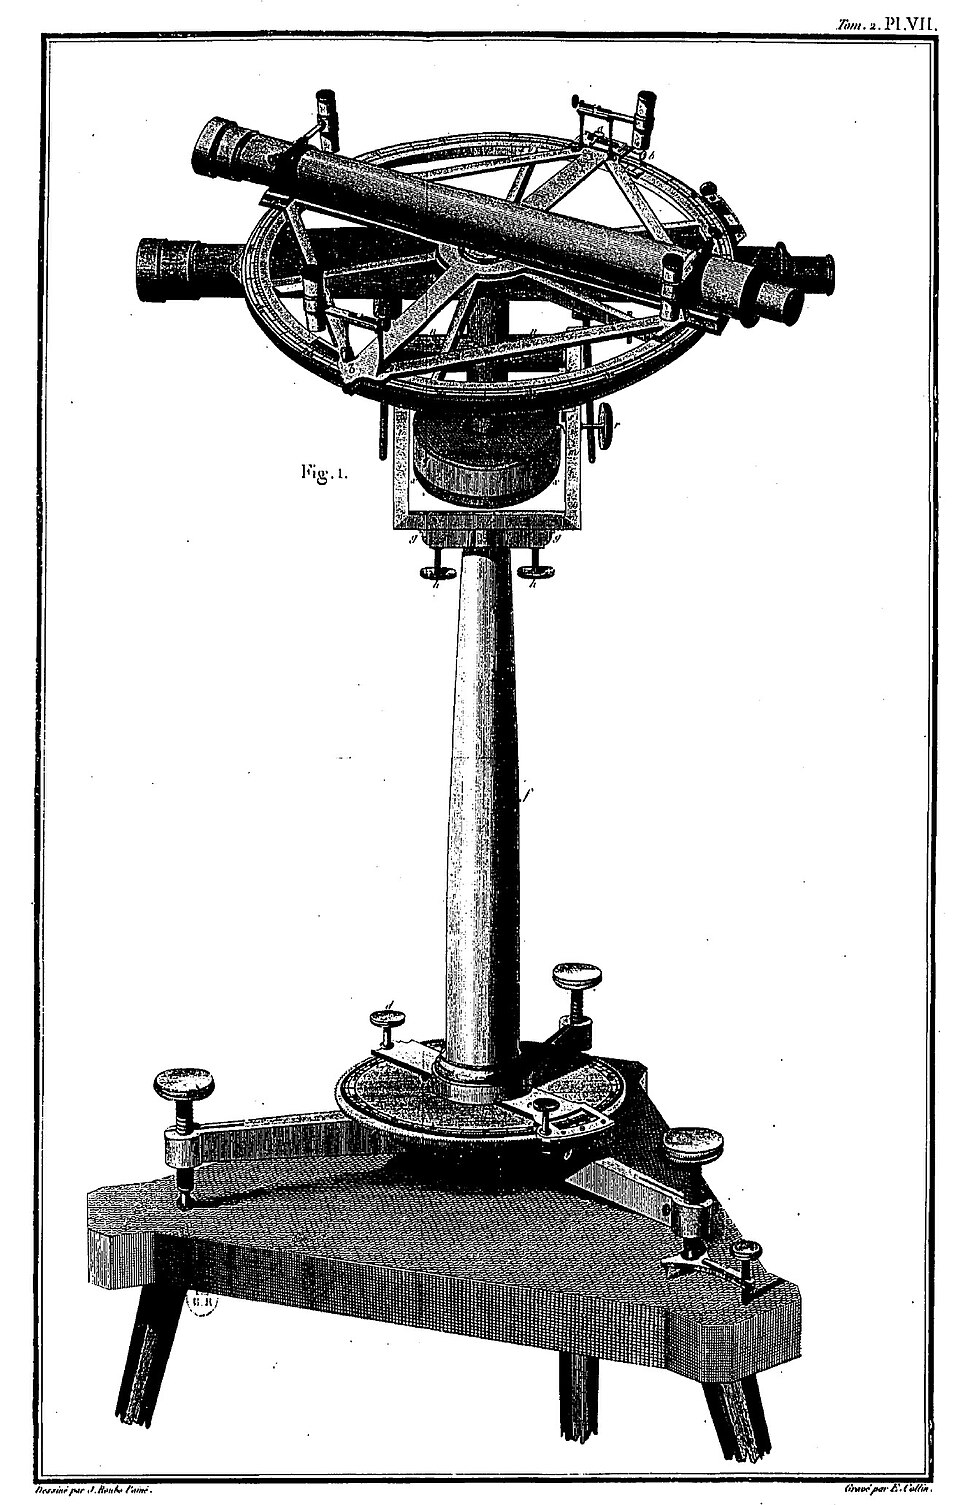
\includegraphics[width=0.3\linewidth]{images/book2/g10-delambre-repeating-circle.jpg}

{\small 用于测量水平角的重复圆仪，如德朗布尔关于此次测量的
记述（1807 年）中所刻的插图。公有领域（
维基共享资源）。}
\end{center}
\end{history}

\section{扁平的地球}

约 1687 年，牛顿依据其万有引力理论论证：自转的地球必为
两极扁平、赤道隆起的椭球体。巴黎天文台的天文学家所测得的
子午线度数似乎表明相反的结论：
地球两极伸长。
这一问题通过测量相距尽可能远的两地之间一度纬度的长度
而得以解决。
% ledger: figure:expeditions

\begin{omfigure}
\begin{tikzpicture}[font=\small, >={Stealth[length=2mm]}]
  \def\a{3.0} \def\b{2.3}
  \draw[black!35, densely dashed] (0,0) circle (\a);
  \fill[omDef!8] (0,0) ellipse ({\a} and {\b});
  \draw[omDef!70!black, thick] (0,0) ellipse ({\a} and {\b});
  \draw[black!50] (-3.4,0) -- (3.7,0);
  \draw[black!50] (0,-2.6) -- (0,3.3);
  \draw[<->, omThm!85!black] (0,-0.3) -- (\a,-0.3);
  \node[omThm!85!black, below] at (1.5,-0.3) {$a$};
  \draw[<->, omThm!85!black] (-0.3,0) -- (-0.3,\b);
  \node[omThm!85!black, left] at (-0.3,1.15) {$b$};
  \node[above right] at (0,\b) {北};
  \node[anchor=south east] at (3.0,-2.5) {};
  \node[anchor=west] at (3.7,0) {赤道};
  % normal at t = 45 deg: P = (2.121, 1.626); crosses the equator at (0.874,0), the axis at (0,-1.14)
  \coordinate (P) at (2.121,1.626);
  \draw[omExo!85!black, thick] (P) -- ($(P)!1.35!(0.874,0)$);
  \draw[omExo!85!black, thick, ->] (P) -- ($(P)!-0.45!(0.874,0)$);
  \fill (P) circle (1.6pt);
  \node[anchor=west, align=left, font=\footnotesize] at (2.85,2.35) {局地竖直线 \\（铅垂线）};
  \draw[omExo!85!black] (1.45,0) arc (0:52.5:0.58);
  \node[omExo!85!black] at (1.62,0.32) {$\varphi$};
  \fill (0,0) circle (1.3pt);
  \node[anchor=north east, font=\footnotesize] at (0,0) {球心};
  \node[black!50, font=\footnotesize, anchor=south] at (-2.2,2.15) {球面};
\end{tikzpicture}

{\small 扁平的地球示意图，\omterm{def:g10:measuring-the-earth:ellipsoid}{扁率}被大幅夸大（真实的\omterm{def:g10:measuring-the-earth:ellipsoid}{扁率}在此比例下过小，
无法看清）。某地的竖直线垂直于地表，
并不严格指向球心。该地的
纬度 $\varphi$ 即其竖直线与
赤道面之间的夹角。}
\end{omfigure}

纬度由恒星观测测得：它是局地竖直线
与赤道面之间的夹角。在扁平的地球上，地表
在两极附近比在赤道附近弯曲得更小。地表越不弯曲，
则沿地表走过的路程必须越长，竖直线才能转过一度：
\emph{纬度一度的长度在两极附近更长}。

\begin{history}[拉普兰与秘鲁]
% ledger: figure:expeditions, figure:degrees
1735 年，巴黎科学院派出一支考察队前往赤道，
地点在西班牙统治下的秘鲁省（今厄瓜多尔）；队员在那里工作了九年，
直至 1744 年。1736--1737 年间，由皮埃尔-路易·莫罗·德·莫佩尔蒂率领的第二支考察队，
与年轻的数学家亚历克西斯·克莱罗一道，测量了子午线上的一度弧长，
地点在拉普兰，靠近北极圈。拉普兰的一度弧长为
57\,437 \emph{托阿兹}（旧长度单位，约合
\qty{111.95}{km}），秘鲁的一度弧长仅为 56\,737 托阿兹：一度弧长在靠近极点处更长，
牛顿是对的。两组数据隐含的\omterm{def:g10:measuring-the-earth:ellipsoid}{扁率}约为
$1/205$——偏大，后来的测量表明如此，但
符号的问题已经得到解决。
\end{history}

\begin{omfigure}
\begin{tikzpicture}
\begin{axis}[omrecord, width=0.82\linewidth, height=5.4cm, xmin=0, xmax=90,
  ymin=110.45, ymax=111.8, xlabel={纬度 (\unit{\degree})},
  ylabel={纬度 \qty{1}{\degree} 的长度 (km)}, xtick={0,15,...,90},
  ytick={110.6,110.8,...,111.8}, yticklabel style={/pgf/number format/fixed, /pgf/number format/fixed zerofill, /pgf/number format/precision=1}]
\addplot[omDef!85!black, line width=1.1pt] table[x=lat_deg, y=deg_km] {figdata/out/grade-10-meridian_degree.dat};
\addplot[only marks, mark=*, mark size=1.8pt, omThm!85!black] coordinates {(0,110.574) (45,111.132) (66,111.507) (90,111.694)};
\node[anchor=south west, font=\footnotesize] at (axis cs:2,110.6) {110.57 km};
\node[anchor=north east, font=\footnotesize] at (axis cs:89,111.56) {111.69 km};
\node[anchor=north west, font=\footnotesize] at (axis cs:46,111.12) {111.13 km};
\node[anchor=south east, font=\footnotesize] at (axis cs:65,111.53) {111.51 km，\ang{66}（拉普兰）};
\end{axis}
\end{tikzpicture}

{\small 纬度一度的长度，取自
\cref{def:g10:measuring-the-earth:ellipsoid}中的\omterm{def:g10:measuring-the-earth:ellipsoid}{参考椭球}，从赤道到极点。
由 WGS~84 椭球计算得出。}
\end{omfigure}

\begin{definition}[参考椭球与扁率]\label{def:g10:measuring-the-earth:ellipsoid}
称\emph{参考椭球}\index{参考椭球}为
由椭圆绕其短轴旋转所得的曲面，选取它是为了尽可能贴合
地球的形状。其\emph{赤道半径}记为
$a$，\emph{极半径}记为 $b$，其
\emph{扁率}\index{扁率}为
\[
  f = \frac{a-b}{a}.
\]
\end{definition}

\begin{proposition}[地球的尺寸]\label{prop:g10:measuring-the-earth:dimensions}
% ledger: wgs84:ellipsoid, earth:Req, earth:Rpol, earth:Rmean (lengths computed in figdata/grade-10/meridian_degree.py)
卫星定位所用的\omterm{def:g10:measuring-the-earth:ellipsoid}{参考椭球}（WGS~84）满足
\[
  a = \qty{6378.137}{km}, \qquad b = \qty{6356.752}{km}, \qquad
  f = \frac{1}{298.257}.
\]
极半径比赤道半径短 \qty{21.4}{km}。赤道
长 \qty{40075}{km}，一条子午线（从一极到另一极再返回）长
\qty{40008}{km}；四分之一子午线，即从赤道到极点的距离，为
\qty{10001.966}{km}。纬度一度在赤道处长 \qty{110.574}{km}，
在两极处长 \qty{111.694}{km}。经度一度在赤道处长
\qty{111.32}{km}，向两极方向缩小，大致按
$\cos \varphi$ 的规律缩短。
\end{proposition}

\begin{example}[经度一度]\label{ex:g10:measuring-the-earth:longitude}
纬度为 $\varphi$ 的纬线是一个圆，其半径为该处到地轴的距离，
约为 $R \cos \varphi$。在北纬 \qty{60}{\degree} 处，其
周长约为赤道的一半，经度一度的长度
约为 $111.32 \times \cos 60^\circ \approx \qty{55.7}{km}$（
椭球计算值为 \qty{55.80}{km}）。
\end{example}

\begin{remark}[地球到底有多圆？]\label{rem:g10:measuring-the-earth:round}
\omterm{def:g10:measuring-the-earth:ellipsoid}{扁率} $1/298$ 很小。直径为 \qty{30}{cm} 的地球仪上，极直径
仅比赤道直径短 \qty{1}{mm}——
肉眼不可见。最深的海沟，位于海平面以下近 \qty{11}{km}，
在这种比例下只是一道深约四分之一毫米的划痕。对大多数用途而言，地球可视为一个
平均半径为 \qty{6371}{km} 的球体；若要精确定位，则需用
椭球。
% ledger: earth:Rmean, usgs:trench-depth
\end{remark}

\section{当今的大地测量学}

\begin{omfigure}
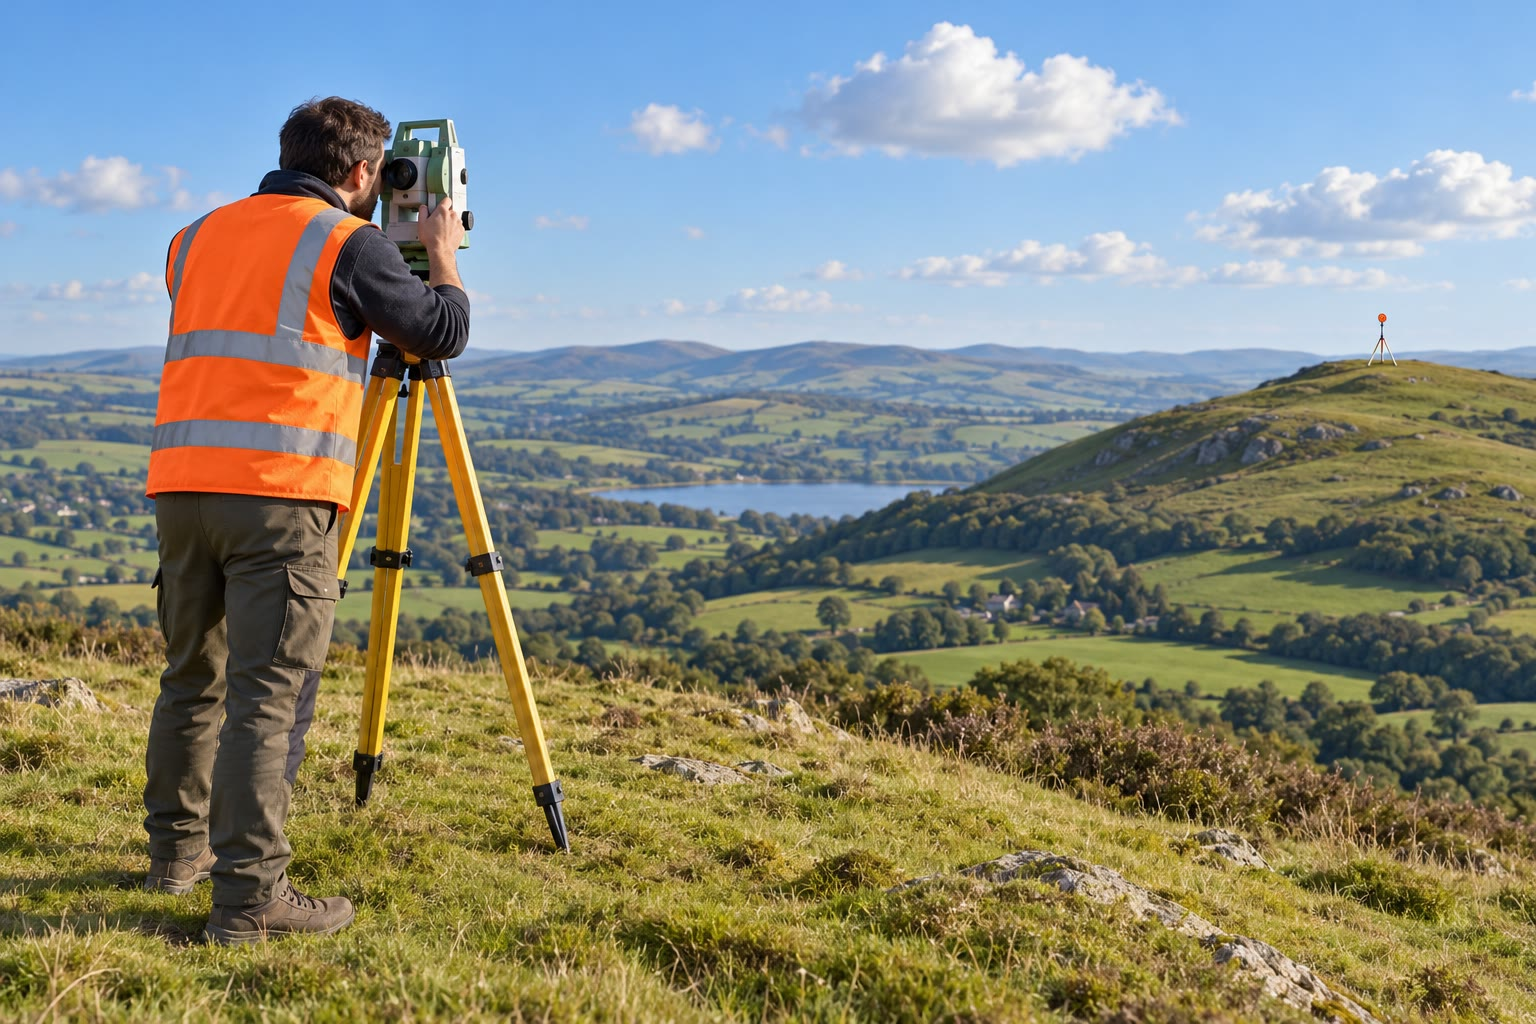
\includegraphics[width=0.7\linewidth]{images/book2/ai/g10-surveyor-theodolite.jpg}

{\small 测量员正在工作，所用的现代仪器可以测量角度，
并借助光束测量距离；远处的
丘陵上立着一座觇标。}
\end{omfigure}

十八、十九世纪的大规模\omterm{def:g10:measuring-the-earth:triangulation}{三角测量}，
已被卫星测量所取代。地面接收机接收
若干颗卫星的信号，这些卫星的位置在每一时刻均已知，
并利用信号的走时计算自身位置（见第 1 册）。
遍布全球、固定于基岩上的常驻接收机组成的网络，
连续测量自身位置。它们确定了
一切地图和卫星位置所依据的参考系，它们本身也在运动：它们
显示岩石圈板块每年漂移数厘米
（见\cref{ch:g11:plate-motions}）。
% ledger: usgs:gps

\begin{inthefield}[今日的地面测量]
\omterm{def:g10:measuring-the-earth:geodesy}{大地测量学}家将天线固定在嵌入基岩的混凝土墩上，远离
建筑物和树木，连续多年每隔数秒记录一次其位置。
他们还将这些结果与射电望远镜的测量数据相结合，后者用于观测
非常遥远的星系，并结合向携带镜子的卫星发射的激光束的测量结果。
测量员在建筑工地和乡村仍用三脚架上的仪器测量角度和
距离，并将其与卫星参考系相衔接。
\end{inthefield}

\section{练习}

\begin{exercise}[$\star$]\label{exo:g10:measuring-the-earth:1}
给出三个无需离开地面即可进行的观察，它们能说明地球是圆的。
对每一个观察，用一句话解释为什么平坦的地球
无法产生这一现象。
\end{exercise}

\begin{exercise}[$\star$]\label{exo:g10:measuring-the-earth:2}
什么是\omterm{def:g10:measuring-the-earth:geodesy}{大地测量学}？什么是\omterm{def:g10:measuring-the-earth:triangulation}{三角测量}？
\omterm{def:g10:measuring-the-earth:triangulation}{三角测量}中需要在地面上测量的是哪一条单独的长度？
\end{exercise}

\begin{exercise}[$\star$]\label{exo:g10:measuring-the-earth:3}
埃拉托色尼发现，当太阳在塞恩正上方时，亚历山大城处太阳光线与
竖直方向的夹角为整圆的 $1/50$，而两城相距 5000 斯塔迪亚。
试以斯塔迪亚为单位计算地球周长，再以千米为单位计算，
取一斯塔迪亚为 \qty{157.2}{m}。
\end{exercise}

\begin{exercise}[$\star$]\label{exo:g10:measuring-the-earth:4}
纬度一度约长 \qty{111}{km}。纬度一分（即一度的 $1/60$）长多少？
从赤道到极点的经线
大约有多长？
\end{exercise}

\begin{exercise}[$\star$]\label{exo:g10:measuring-the-earth:5}
已知赤道半径为 \qty{6378.137}{km}，极半径为
\qty{6356.752}{km}，求两半径之差以及\omterm{def:g10:measuring-the-earth:ellipsoid}{扁率} $f = (a-b)/a$。
将 $f$ 写成 1 除以一个整数的形式。
\end{exercise}

\begin{exercise}[$\star\star$]\label{exo:g10:measuring-the-earth:6}
两座城镇位于同一条经线上，相距 \qty{500}{km}。同一天正午，
竖直立着的一根高 \qty{1.00}{m} 的标杆，在南方城镇的影子长 \qty{0.364}{m}，
在北方城镇的影子长 \qty{0.456}{m}。
求两城中太阳光线与竖直方向的夹角，
再求地球的周长。
\end{exercise}

\begin{exercise}[$\star\star$]\label{exo:g10:measuring-the-earth:7}
在三角形 $ABC$ 中，基线 $AB = \qty{10.00}{km}$，$A$ 处的角为
\qty{62}{\degree}，$B$ 处的角为 \qty{71}{\degree}。求
$C$ 处的角以及边长 $AC$ 和 $BC$。
\end{exercise}

\begin{exercise}[$\star\star$]\label{exo:g10:measuring-the-earth:8}
一架飞机沿北纬 \qty{60}{\degree} 纬线正西向飞行，
经度从东经 \qty{10}{\degree} 变至西经 \qty{20}{\degree}。
取经度一度的长度为 $111.3 \cos \varphi$ 千米，求其飞过的距离。
同样的经度变化在赤道上会是多长？
\end{exercise}

\begin{exercise}[$\star\star$]\label{exo:g10:measuring-the-earth:9}
观察者的眼睛位于平静海面上方 $h = \qty{2}{m}$ 处。到地平线的视线恰好擦过海面上的点 $T$，
地球中心为 $O$，眼睛所在位置为 $E$。解释为何三角形 $OTE$ 在 $T$ 处为直角，
再利用毕达哥拉斯定理，取 $R = \qty{6371}{km}$，
证明到地平线的距离约为 $\sqrt{2Rh}$，
并计算其值。
\end{exercise}

\begin{exercise}[$\star\star$]\label{exo:g10:measuring-the-earth:10}
读取度长曲线。纬度一度的长度在哪两个纬度之间
变化最快？用两句话解释，
为什么纬度一度的长度在极地附近比在赤道附近更长。
\end{exercise}

\begin{exercise}[$\star\star$]\label{exo:g10:measuring-the-earth:11}
从敦刻尔克到巴塞罗那的子午弧跨越纬度 \qty{9.646}{\degree}，
长 \qty{1072.2}{km}。求该弧段上纬度一度的平均长度。
若每一度都取这一长度，四分之一子午线会有多长？
将其与 \qty{10002.0}{km} 比较，
并解释两者的微小差异。
\end{exercise}

\begin{exercise}[$\star\star\star$]\label{exo:g10:measuring-the-earth:12}
埃拉托色尼测得角度为 \qty{7.2}{\degree}，距离为 5000 斯塔迪亚。
若他的角度偏小了 \qty{0.1}{\degree}，
周长的误差为百分之几，误差方向如何？
你认为他的两次测量中哪一次精度较低？
\end{exercise}

\begin{exercise}[$\star\star\star$]\label{exo:g10:measuring-the-earth:13}
由两个三角形组成的链：在 $ABC$ 中，$AB = \qty{6.000}{km}$，
$A = \qty{55}{\degree}$，$B = \qty{75}{\degree}$。在下一个三角形 $ACD$ 中，
它建立在边 $AC$ 上，$A$ 处的角为 \qty{50}{\degree}，$C$ 处的角为
\qty{68}{\degree}。求 $AC$，再求 $AD$。
\end{exercise}

\begin{exercise}[$\star\star\star$]\label{exo:g10:measuring-the-earth:14}
在哪个纬度上，经度一度的长度是赤道上的一半？
在哪个纬度上，它是赤道上的十分之一？
请解释为何这两个答案都与地球的大小无关。
\end{exercise}

\begin{exercise}[$\star\star\star$]\label{exo:g10:measuring-the-earth:15}
利用椭球的数值：纬度一度在赤道处长 \qty{110.574}{km}，
在极点处长 \qty{111.694}{km}。若取平均半径相同的球体，
则一度处处为 \qty{111.195}{km}。假设地球为球体的测量员，
在赤道上的一度与在极点上的一度，分别会偏差多少米？
为何要精确到米的地图必须在
椭球上计算？
\end{exercise}

\section{问题：米与子午线}

\begin{problem}[{周末问题——从埃拉托色尼的影子
到第一米的长度}]
\label{pb:g10:measuring-the-earth:1}
% ledger: geonames:aswan, geonames:alexandria, erat:method, metre:1791, metre:survey, wgs84:ellipsoid (arc lengths and degree lengths computed in figdata/grade-10/meridian_degree.py)
一名学生用现代数据，重新梳理地球测量的历史。阿斯旺（古代的塞恩）
位于北纬 \qty{24.09}{\degree}，亚历山大位于北纬 \qty{31.20}{\degree}。
在现代椭球上，两地纬线之间的子午弧长为 \qty{788}{km}。
在椭球上，纬度一度在赤道处长 \qty{110.57}{km}，
在 \qty{45}{\degree} 处长 \qty{111.13}{km}，
在 \qty{66}{\degree} 处长 \qty{111.51}{km}，
四分之一子午线长
\qty{10001.966}{km}。

\medskip
\noindent\textbf{第一部分——再谈埃拉托色尼。}
\begin{enumerate}
  \item 计算阿斯旺与亚历山大之间的纬度差。
  \item 它占整个圆周的几分之几？将其与埃拉托色尼的
        $1/50$ 作比较。
  \item 用这些现代数据，计算按埃拉托色尼的方法
        所得的地球周长。
  \item 两城市不在同一经线上：阿斯旺位于亚历山大以东约
        \qty{3}{\degree} 经度处。本方法中必须使用哪一段距离：
        两城市之间的直线距离，还是
        两者纬线之间的子午线弧长？为什么？
  \item 为什么两处的影子必须在同一天、当地正午测量？
\end{enumerate}

\medskip
\noindent\textbf{第二部分——小型\omterm{def:g10:measuring-the-earth:triangulation}{三角测量}。}
测得基线 $AB = \qty{12.000}{km}$。从 $A$ 处观测到信号 $C$，
视线与 $B$ 方向的夹角为 \qty{58}{\degree}；从 $B$ 处看，视线与 $A$ 方向的夹角为 \qty{66}{\degree}。
在下一个三角形 $ACD$ 中，$A$ 处的角为 \qty{47}{\degree}，
$C$ 处的角为 \qty{75}{\degree}。边 $AD$ 指向
北偏东 \qty{8}{\degree}。
\begin{enumerate}[resume]
  \item 求 $C$ 处的角（三角形 $ABC$ 中）。
  \item 求边 $AC$。
  \item 求边 $BC$。
  \item 求 $D$ 处的角（三角形 $ACD$ 中），再求边 $AD$。
  \item 求 $A$、$D$ 两点之间的南北距离。
  \item 利用 \qty{45}{\degree} 处每度的长度，计算
        $A$、$D$ 两点之间的纬度差，分别以度和
        角分表示。
\end{enumerate}

\medskip
\noindent\textbf{第三部分——扁球形的地球。}
\begin{enumerate}[resume]
  \item 纬度 \qty{66}{\degree} 处一度纬度的长度比赤道处的
        一度长多少米？
  \item 解释这一差异说明地球的形状有何特点。
  \item 在椭球体上，$a = \qty{6378.137}{km}$，
        $b = \qty{6356.752}{km}$。计算 $a - b$ 及\omterm{def:g10:measuring-the-earth:ellipsoid}{扁率}。
  \item 解释为什么在扁球形地球上，纬度
        \qty{45}{\degree} 处的铅垂线并不恰好指向
        地心。
\end{enumerate}

\medskip
\noindent\textbf{第四部分——第一米。}
\begin{enumerate}[resume]
  \item 按照 1791 年的定义，四分之一子午线
        应为多少米？
  \item 1799 年的铂质米尺是根据子午线的
        一个测量值制成的。若四分之一子午线实际长为 \qty{10001.966}{km}，
        则其千万分之一是多长？
  \item 1799 年的米尺与其自身的定义相比，是偏长
        还是偏短？相差的比例为多少？
  \item 铂质米尺忠实地复制了 1790 年代计算的长度。
        当时计算出的四分之一子午线是偏长还是偏短？
        请说明理由。
  \item 第一米比真实四分之一子午线的千万分之一
        短了多少毫米？可与一张纸的
        厚度作比较：纸厚约 \qty{0.1}{mm}。
\end{enumerate}
\end{problem}
